\documentclass[tikz,border=20pt]{standalone}
\usepackage{helvet}
\renewcommand{\familydefault}{\sfdefault}
\usetikzlibrary{positioning, fit, backgrounds, arrows.meta, shapes.geometric, calc}
\usepackage{pagecolor}

\definecolor{azblue}{HTML}{0078D4}
\definecolor{azdark}{HTML}{0F172A}
\definecolor{azlight}{HTML}{F0F6FF}
\definecolor{copper}{HTML}{B87333}

\begin{document}
\pagecolor{white}
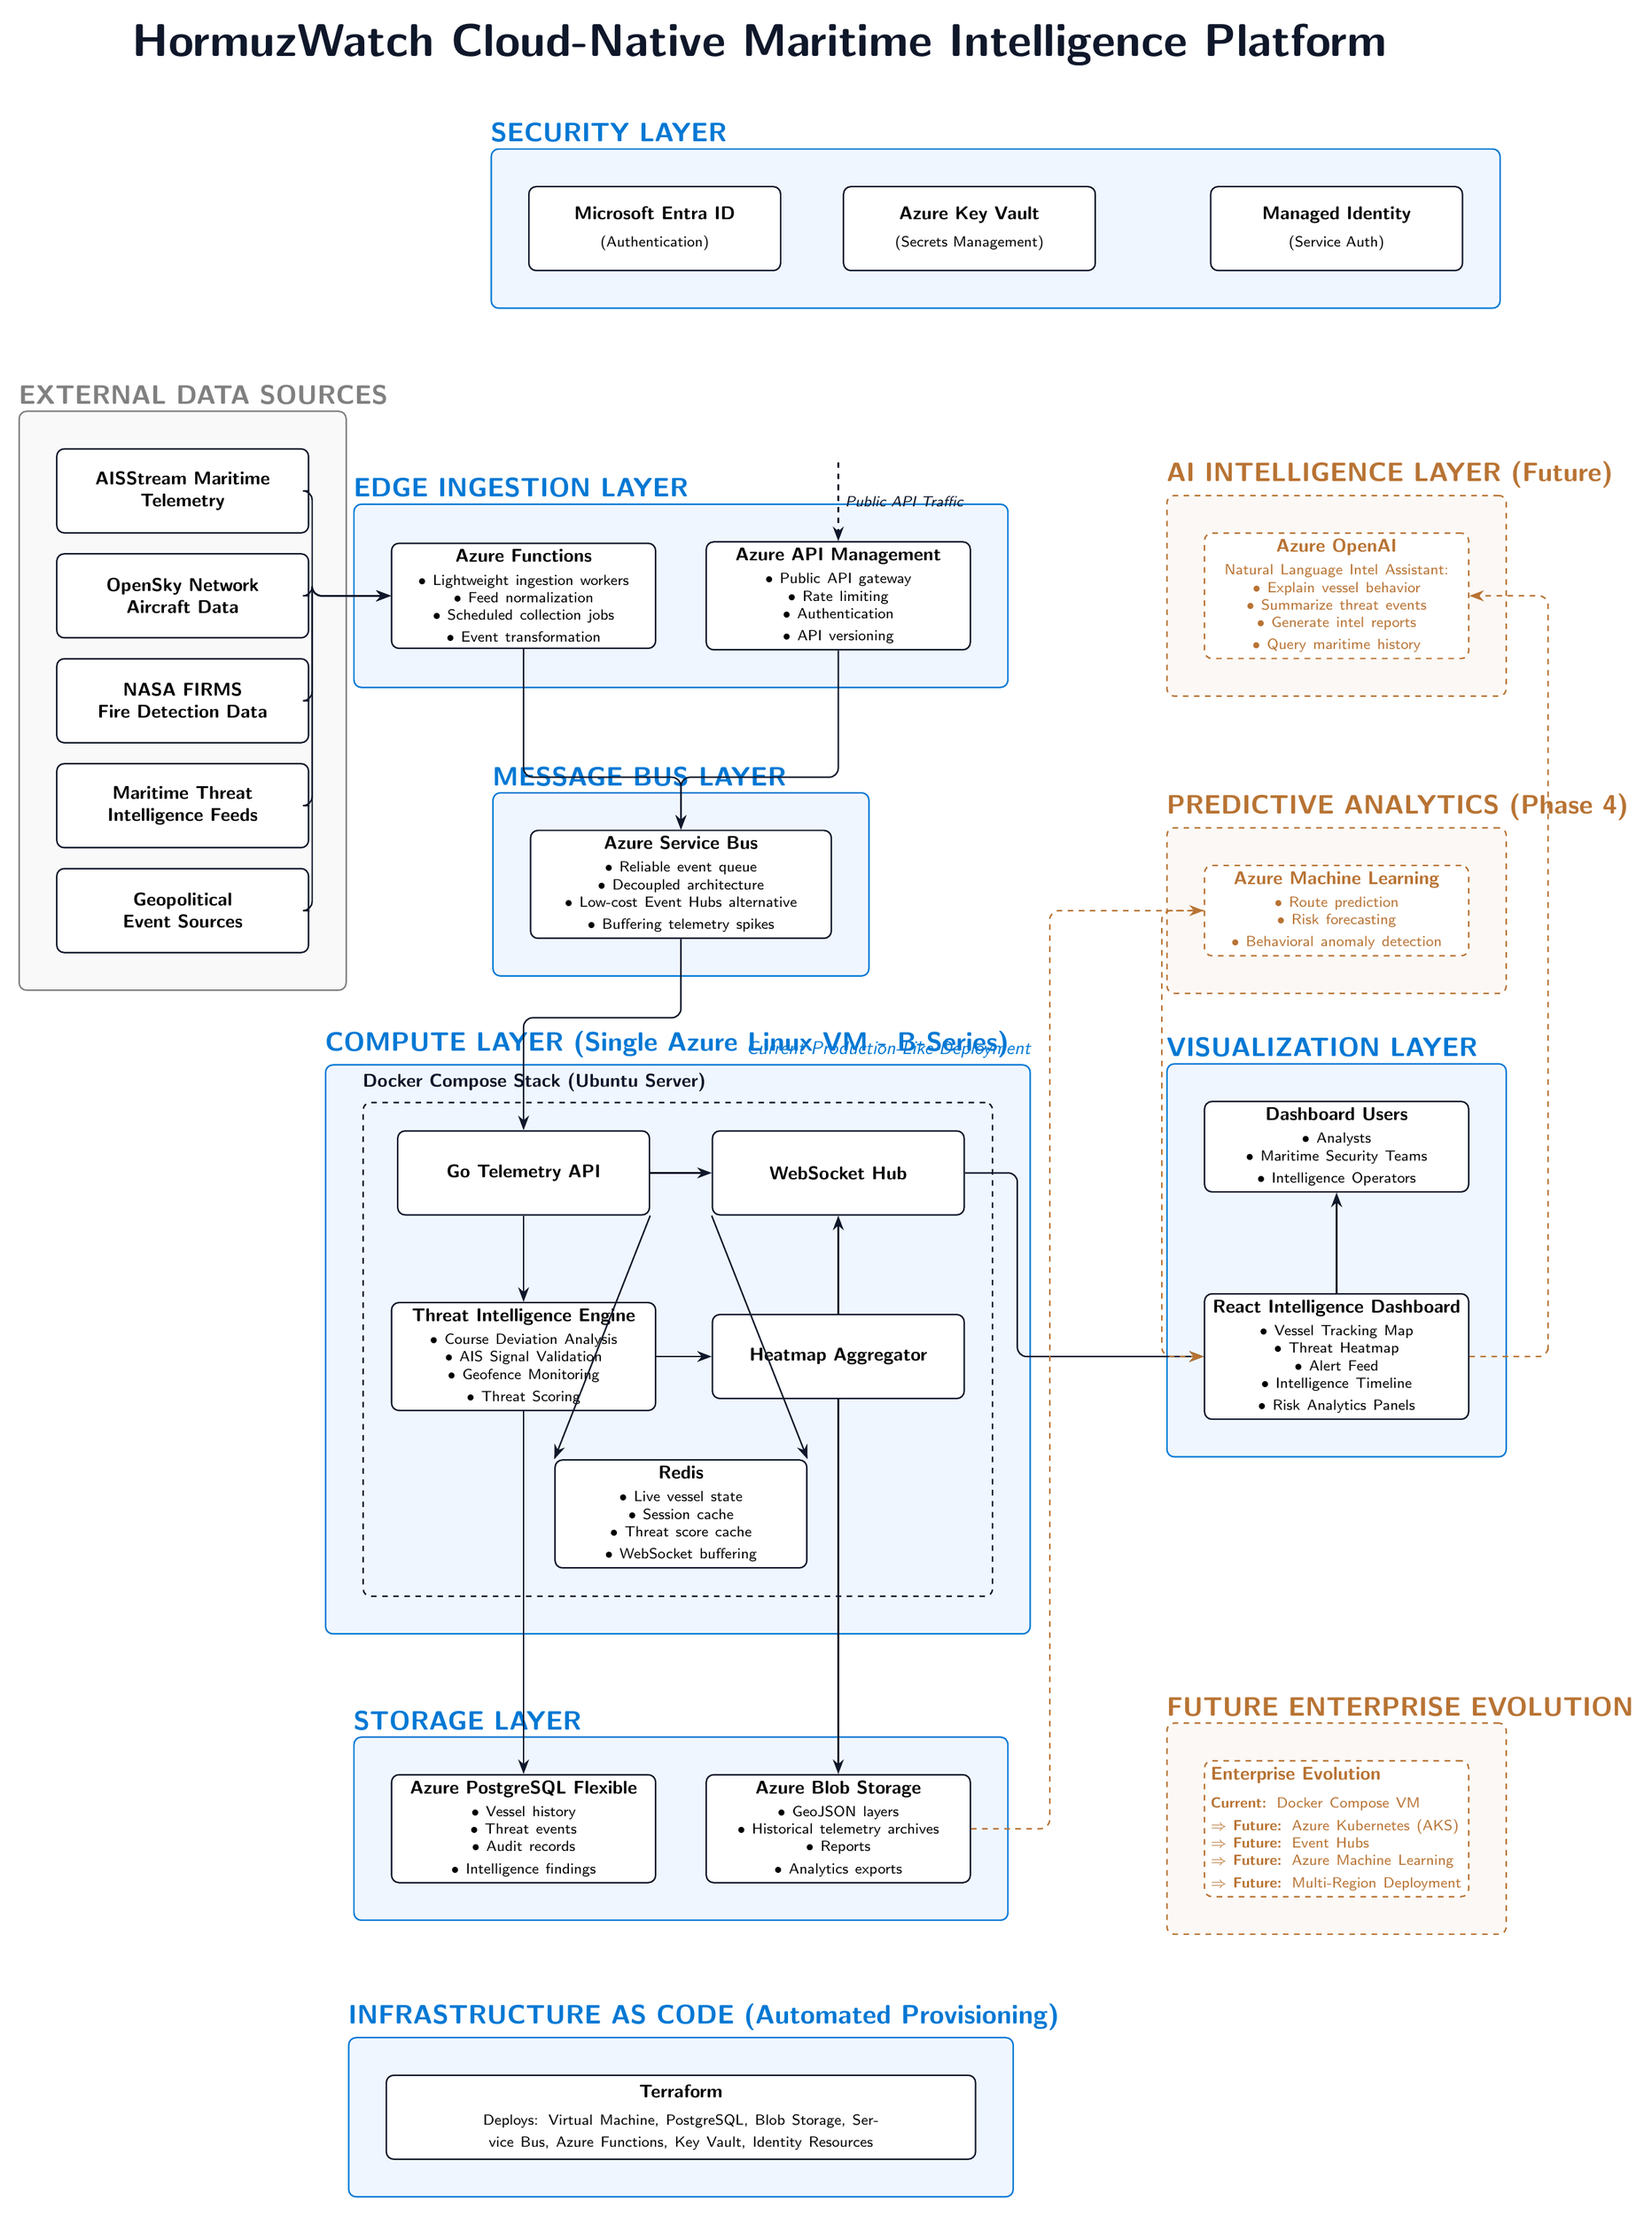
\begin{tikzpicture}[
    font=\sffamily,
    % Box styles
    layerbox/.style={rectangle, draw=azblue, thick, rounded corners, inner sep=20pt, fill=azlight},
    extlayerbox/.style={rectangle, draw=gray, thick, rounded corners, inner sep=20pt, fill=gray!5},
    futurelayerbox/.style={rectangle, draw=copper, thick, dashed, rounded corners, inner sep=20pt, fill=copper!5},
    resourcebox/.style={rectangle, draw=azdark, thick, rounded corners, fill=white, minimum width=4.8cm, minimum height=1.6cm, align=center, font=\bfseries},
    futurebox/.style={rectangle, draw=copper, thick, dashed, rounded corners, fill=white, minimum width=4.8cm, minimum height=1.6cm, align=center, font=\bfseries\color{copper}},
    layerlabel/.style={font=\Large\bfseries\color{azblue}, anchor=south west, inner xsep=0pt},
    extlayerlabel/.style={font=\Large\bfseries\color{gray}, anchor=south west, inner xsep=0pt},
    futurelayerlabel/.style={font=\Large\bfseries\color{copper}, anchor=south west, inner xsep=0pt},
    arrow/.style={-{Stealth[scale=1.2]}, thick, azdark},
    dashedarrow/.style={-{Stealth[scale=1.2]}, thick, dashed, copper}
]

% ==================== TITLE ====================
\node[font=\Huge\bfseries\color{azdark}, align=center] (title) at (11, 8.5) {HormuzWatch Cloud-Native Maritime Intelligence Platform};

% ==================== 1. EXTERNAL DATA SOURCES ====================
\node[resourcebox] (ext1) at (0, 0) {AISStream Maritime\\Telemetry};
\node[resourcebox] (ext2) at (0, -2) {OpenSky Network\\Aircraft Data};
\node[resourcebox] (ext3) at (0, -4) {NASA FIRMS\\Fire Detection Data};
\node[resourcebox] (ext4) at (0, -6) {Maritime Threat\\Intelligence Feeds};
\node[resourcebox] (ext5) at (0, -8) {Geopolitical\\Event Sources};

\begin{scope}[on background layer]
    \node[fit=(ext1) (ext5), extlayerbox] (extlayer) {};
\end{scope}
\node[extlayerlabel] at (extlayer.north west) {EXTERNAL DATA SOURCES};

% ==================== 2. SECURITY LAYER ====================
\node[resourcebox] (entra) at (9, 5) {Microsoft Entra ID\\[1mm] \normalfont\footnotesize (Authentication)};
\node[resourcebox] (kv) at (15, 5) {Azure Key Vault\\[1mm] \normalfont\footnotesize (Secrets Management)};
\node[resourcebox] (mi) at (22, 5) {Managed Identity\\[1mm] \normalfont\footnotesize (Service Auth)};

\begin{scope}[on background layer]
    \node[fit=(entra) (kv) (mi), layerbox] (seclayer) {};
\end{scope}
\node[layerlabel] at (seclayer.north west) {SECURITY LAYER};

% ==================== 3. EDGE INGESTION LAYER ====================
\node[resourcebox, text width=4.8cm] (functions) at (6.5, -2) {Azure Functions\\[1mm] \normalfont\footnotesize $\bullet$ Lightweight ingestion workers\\ $\bullet$ Feed normalization\\ $\bullet$ Scheduled collection jobs\\ $\bullet$ Event transformation};
\node[resourcebox, text width=4.8cm] (apim) at (12.5, -2) {Azure API Management\\[1mm] \normalfont\footnotesize $\bullet$ Public API gateway\\ $\bullet$ Rate limiting\\ $\bullet$ Authentication\\ $\bullet$ API versioning};

\begin{scope}[on background layer]
    \node[fit=(apim) (functions), layerbox] (edgelayer) {};
\end{scope}
\node[layerlabel] at (edgelayer.north west) {EDGE INGESTION LAYER};

% ==================== 4. MESSAGE BUS LAYER ====================
\node[resourcebox, text width=5.5cm] (servicebus) at (9.5, -7.5) {Azure Service Bus\\[1mm] \normalfont\footnotesize $\bullet$ Reliable event queue\\ $\bullet$ Decoupled architecture\\ $\bullet$ Low-cost Event Hubs alternative\\ $\bullet$ Buffering telemetry spikes};

\begin{scope}[on background layer]
    \node[fit=(servicebus), layerbox] (buslayer) {};
\end{scope}
\node[layerlabel] at (buslayer.north west) {MESSAGE BUS LAYER};

% ==================== 5. COMPUTE LAYER ====================
\node[resourcebox] (goapi) at (6.5, -13) {Go Telemetry API};
\node[resourcebox] (wshub) at (12.5, -13) {WebSocket Hub};
\node[resourcebox, text width=4.8cm] (anomaly) at (6.5, -16.5) {Threat Intelligence Engine\\[1mm] \normalfont\footnotesize $\bullet$ Course Deviation Analysis\\ $\bullet$ AIS Signal Validation\\ $\bullet$ Geofence Monitoring\\ $\bullet$ Threat Scoring};
\node[resourcebox] (heatmap) at (12.5, -16.5) {Heatmap Aggregator};
\node[resourcebox, text width=4.5cm] (redis) at (9.5, -19.5) {Redis\\[1mm] \normalfont\footnotesize $\bullet$ Live vessel state\\ $\bullet$ Session cache\\ $\bullet$ Threat score cache\\ $\bullet$ WebSocket buffering};

% Docker Compose Boundary
\node[fit=(goapi) (wshub) (anomaly) (heatmap) (redis), rectangle, draw=azdark, dashed, thick, inner sep=15pt, rounded corners] (docker) {};
\node[anchor=south west, font=\bfseries\color{azdark}, inner xsep=0pt, yshift=2pt] at (docker.north west) {Docker Compose Stack (Ubuntu Server)};

\begin{scope}[on background layer]
    \node[fit=(docker), layerbox] (computelayer) {};
\end{scope}
\node[layerlabel] at (computelayer.north west) {COMPUTE LAYER (Single Azure Linux VM - B-Series)};
\node[anchor=south east, font=\itshape\color{azblue}, inner xsep=0pt] at (computelayer.north east) {Current Production-Like Deployment};

% ==================== 6. STORAGE LAYER ====================
\node[resourcebox, text width=4.8cm] (pg) at (6.5, -25.5) {Azure PostgreSQL Flexible\\[1mm] \normalfont\footnotesize $\bullet$ Vessel history\\ $\bullet$ Threat events\\ $\bullet$ Audit records\\ $\bullet$ Intelligence findings};
\node[resourcebox, text width=4.8cm] (blob) at (12.5, -25.5) {Azure Blob Storage\\[1mm] \normalfont\footnotesize $\bullet$ GeoJSON layers\\ $\bullet$ Historical telemetry archives\\ $\bullet$ Reports\\ $\bullet$ Analytics exports};

\begin{scope}[on background layer]
    \node[fit=(pg) (blob), layerbox] (storagelayer) {};
\end{scope}
\node[layerlabel] at (storagelayer.north west) {STORAGE LAYER};

% ==================== 7. IAC LAYER ====================
\node[resourcebox, text width=11cm] (tf) at (9.5, -31) {Terraform\\[1mm] \normalfont\footnotesize Deploys: Virtual Machine, PostgreSQL, Blob Storage, Service Bus, Azure Functions, Key Vault, Identity Resources};

\begin{scope}[on background layer]
    \node[fit=(tf), layerbox] (iaclayer) {};
\end{scope}
\node[layerlabel] at (iaclayer.north west) {INFRASTRUCTURE AS CODE (Automated Provisioning)};

% ==================== 8. AI INTELLIGENCE LAYER (Future) ====================
\node[futurebox, text width=4.8cm] (openai) at (22, -2) {Azure OpenAI\\[1mm] \normalfont\footnotesize Natural Language Intel Assistant:\\ $\bullet$ Explain vessel behavior\\ $\bullet$ Summarize threat events\\ $\bullet$ Generate intel reports\\ $\bullet$ Query maritime history};

\begin{scope}[on background layer]
    \node[fit=(openai), futurelayerbox] (ailayer) {};
\end{scope}
\node[futurelayerlabel] at (ailayer.north west) {AI INTELLIGENCE LAYER (Future)};

% ==================== 9. PREDICTIVE ANALYTICS LAYER (Future) ====================
\node[futurebox, text width=4.8cm] (aml) at (22, -8) {Azure Machine Learning\\[1mm] \normalfont\footnotesize $\bullet$ Route prediction\\ $\bullet$ Risk forecasting\\ $\bullet$ Behavioral anomaly detection};

\begin{scope}[on background layer]
    \node[fit=(aml), futurelayerbox] (mllayer) {};
\end{scope}
\node[futurelayerlabel] at (mllayer.north west) {PREDICTIVE ANALYTICS (Phase 4)};

% ==================== 10. VISUALIZATION LAYER ====================
\node[resourcebox, text width=4.8cm] (users) at (22, -12.5) {Dashboard Users\\[1mm] \normalfont\footnotesize $\bullet$ Analysts\\ $\bullet$ Maritime Security Teams\\ $\bullet$ Intelligence Operators};
\node[resourcebox, text width=4.8cm] (react) at (22, -16.5) {React Intelligence Dashboard\\[1mm] \normalfont\footnotesize $\bullet$ Vessel Tracking Map\\ $\bullet$ Threat Heatmap\\ $\bullet$ Alert Feed\\ $\bullet$ Intelligence Timeline\\ $\bullet$ Risk Analytics Panels};

\begin{scope}[on background layer]
    \node[fit=(users) (react), layerbox] (vislayer) {};
\end{scope}
\node[layerlabel] at (vislayer.north west) {VISUALIZATION LAYER};

% ==================== 11. FUTURE ENTERPRISE EVOLUTION ====================
\node[futurebox, text width=4.8cm, align=left] (evolution) at (22, -25.5) {\textbf{Enterprise Evolution}\\[2mm] \normalfont\footnotesize \textbf{Current:} Docker Compose VM\\[1mm] $\Rightarrow$ \textbf{Future:} Azure Kubernetes (AKS)\\ $\Rightarrow$ \textbf{Future:} Event Hubs\\ $\Rightarrow$ \textbf{Future:} Azure Machine Learning\\ $\Rightarrow$ \textbf{Future:} Multi-Region Deployment};

\begin{scope}[on background layer]
    \node[fit=(evolution), futurelayerbox] (evolayer) {};
\end{scope}
\node[futurelayerlabel] at (evolayer.north west) {FUTURE ENTERPRISE EVOLUTION};


% ==================== ROUTING ARROWS ====================

% External to Edge
\coordinate (ingestpoint) at ($(functions.west) + (-1.5, 0)$);
\foreach \i in {1,2,3,4,5} {
    \draw[arrow, rounded corners=5pt] (ext\i.east) -| (ingestpoint) |- (functions.west);
}

% Public to APIM
\coordinate (publicapi) at ($(apim.north) + (0, 1.5)$);
\draw[arrow, dashed] (publicapi) -- (apim.north) node[midway, right, font=\footnotesize\itshape] {Public API Traffic};

% Edge to Bus
\draw[arrow, rounded corners=5pt] (functions.south) |- ($(servicebus.north) + (0, 1)$) -- (servicebus.north);
\draw[arrow, rounded corners=5pt] (apim.south) |- ($(servicebus.north) + (0, 1)$) -- (servicebus.north);

% Bus to Compute
\draw[arrow, rounded corners=5pt] (servicebus.south) -- ++(0,-1.5) -| (goapi.north);

% Compute Internals
\draw[arrow] (goapi.south) -- (anomaly.north);
\draw[arrow] (anomaly.east) -- (heatmap.west);
\draw[arrow] (heatmap.north) -- (wshub.south);
\draw[arrow] (goapi.east) -- (wshub.west);
\draw[arrow] (goapi.south east) -- (redis.north west);
\draw[arrow] (wshub.south west) -- (redis.north east);

% Compute to Storage
\draw[arrow] (anomaly.south) -- (pg.north);
\draw[arrow] (heatmap.south) -- (blob.north);

% Visualization
\draw[arrow, rounded corners=5pt] (wshub.east) -- ++(1,0) |- (react.west);
\draw[arrow] (react.north) -- (users.south);

% ML Flows
\draw[dashedarrow, rounded corners=5pt] (blob.east) -- ++(1.5,0) |- (aml.west);
\draw[dashedarrow, rounded corners=5pt] (aml.west) -| ++(-0.8, -4) |- (react.west);

% OpenAI Flows
\draw[dashedarrow, rounded corners=5pt] (react.east) -| ++(1.5, 0) |- (openai.east);

\end{tikzpicture}
\end{document}
